
\section{Ohm's Law}

Name \rule{2.0in}{0.1pt}\hfill{}Section \rule{1.0in}{0.1pt}\hfill{}Date
\rule{1.0in}{0.1pt}

\textbf{Objectives}

\begin{itemize}
\item To investigate the most important principle in electronics.
\item To determine how resistors in series and parallel add.
\end{itemize}
\textbf{Introduction}

The rate at which electric charge flows through a conductor is called
the electric current. In order to have a current, a potential difference,
or voltage is necessary. We first want to determine the relationship
between the potential difference at two ends of a conductor and the
current flowing through it.

\textbf{Note}: Do not turn on a power supply until you are sure your
circuit is correct. If you are at all unsure, please ask your instructor
to approve your setup. Ammeters can be instantly and permanently ruined
by an improper connection. Be sure to turn off the power supply before
making any changes to the circuit.

\textbf{Apparatus}

\begin{itemize}
\item Power supply
\item Two resistors
\item Leads and alligator clips
\item DC Milliammeter
\item Multimeter
\end{itemize}
\textbf{Activity 1: Ohm's Law}

\begin{itemize}
%\item Connect two rheostats (or variable resistors) in series as shown in
%the figure below. Set R\( _{1} \) at about the halfway point and
%R\( _{2} \) at the maximum. Connect an ammeter as shown. Also, connect
%a voltmeter across (that is, connect a probe to each side of) R\( _{1} \).
%\item The fixed resistor will be considered an ``unknown'' and will be called 
%R\( _{1} \). The variable resistor will be called R\( _{2} \), and will be used 
%to vary the current. Connect the two resistors in series as shown in the 
%figure. Set R\( _{2} \) at its maximum value. Connect a milliammeter as shown, 
%at the point marked ``A'' (for ``ammeter''). Leave the positive lead to the 
%power supply disconnected.
\item With the power supply off, turn the coarse current control all the way up 
and both voltage controls all the way down.  Connect one of the resistors in 
series with the milliammeter (marked ``A'' for ``ammeter'') as shown in the 
figure below. Be sure the polarity of the milliammeter is as shown.
\end{itemize}
\vspace{0.3cm}
{\centering \resizebox*{0.35\textwidth}{!}{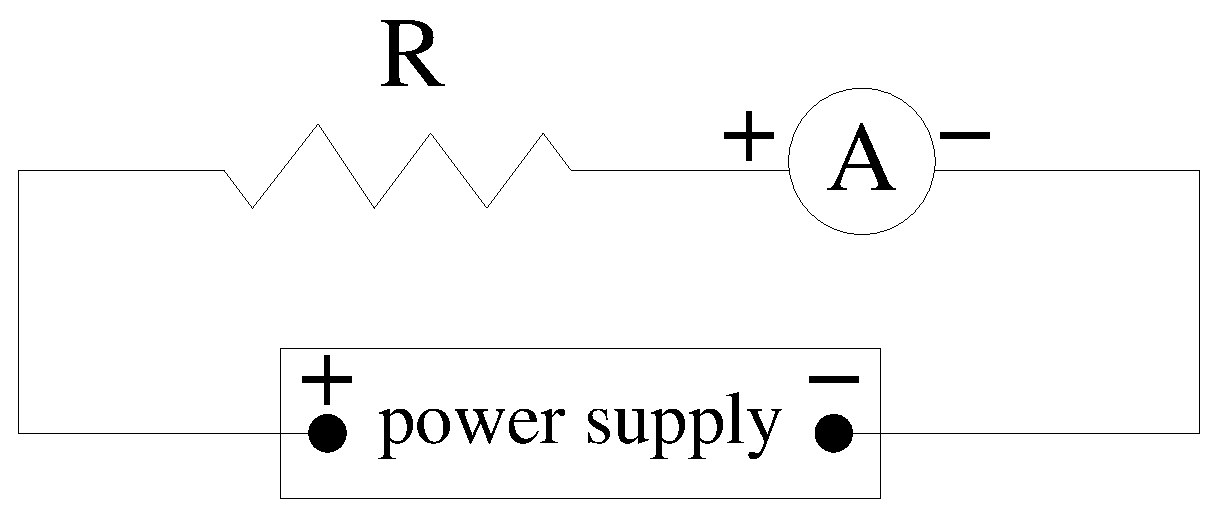
\includegraphics{ohms_law/ohms_law_fig_3.eps}} \par}
\vspace{0.3cm}

\begin{itemize}
\item When sure of your circuit, turn on the power supply, and turn the coarse 
voltage control up until the milliammeter reads 20 ma. Measure the voltage 
across the resistor (with the multimeter set for DC voltage) and record both voltage and current here. Include an uncertainty in the voltage measurement.
\vspace{10mm}

%\item Reduce the resistance of R\( _{2} \) and record the current and voltage
%three more times by turning down R\( _{2} \) in approximately equal steps so 
%that for the last time R\( _{2} \) is turned completely down. 
%Record your results here:\vspace{30mm}

\item Now turn the coarse voltage control up and record current and voltage 
for four more values of current: 40, 60, 80, and 100 ma. Include uncertainties
 in the voltage measurements.
\vspace{30mm}

\item Turn off the power supply.

\item Using $Excel$, plot your five pairs of readings with the voltage on the 
vertical axis and the current on the horizontal axis. Include the origin as a 
sixth point (why is this valid?).
\vspace{6mm}
\item Fit a straight line to the points (including the origin).
Include a trendline with equation.
\item Use the LINEST function in $Excel$ (see \textbf{Appendix C}) to 
determine the slope of the line and its uncertainty.  What is the meaning 
of the slope? Write its value with uncertainty here (including units):
\vspace{20mm}

\item Print the graph and include it with this unit.

\item Remove the resistor from the rest of the circuit and use the ohmmeter
option on the multimeter to measure the resistance of R directly.
Does it fall within the range of values determined above? Can you think of 
a reason for any discrepancy?
\vspace{20mm}

\item What is the general relationship between voltage, current, and resistance?
This is Ohm's Law.\vspace{15mm}

\item Why is the origin a legitimate point on the curve?\vspace{15mm}

\end{itemize}
\textbf{Activity 2: Resistors in Series}

\begin{itemize}
%\item Turn rheostat R\( _{2} \) to its maximum setting. Connect the multimeter
%across this resistor, being sure to set it for reading voltages.
%\item When you are sure the circuit is set, turn on the power supply and
%record the current and voltage. Turn off the power supply.\vspace{10mm}

%\item \textbf{Prediction}: Based on your measurements, predict the resistance
%of R\( _{2} \).\vspace{15mm}

%\item Remove and measure the resistance of R\( _{2} \). Record the percent
%difference between your prediction and measurement. Replace R\( _{2} \).\vspace{30mm}

%\item Was the current this time different from the first reading in Activity
%1?\vspace{15mm}

\item Turn the voltage control down to zero, and connect two resistors in 
series as shown in the figure below.
\end{itemize}
\vspace{0.3cm}
{\centering \resizebox*{0.35\textwidth}{!}{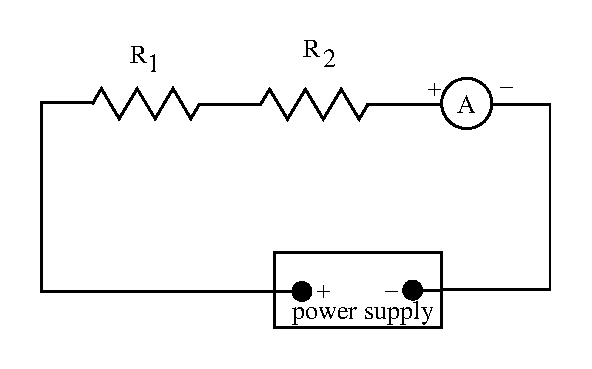
\includegraphics{ohms_law/ohms_law_fig_1.eps}} \par}
\vspace{0.3cm}

\begin{itemize}

\item Turn on the power supply and turn up the coarse voltage control to 
approximately 10 volts. Measure the voltages across R\( _{1} \), R\( _{2} \), 
and the milliammeter. (The voltage across the milliammeter may be in \underline{millivolts}.) Also measure the total voltage across all three elements 
in series. Include uncertainties in each measurement. Record your results here:
\vspace{20mm}

\item How is the last measurement related to the three individual 
measurements?
\vspace{10mm}

\item What can you conclude about the voltage across resistors in series?
\vspace{10mm}

\item Measure the current in the series circuit and record it here:
\vspace{10mm}

\item Using Ohm's Law, determine the total resistance of the circuit from the 
total voltage and the current which you have measured.
\vspace{10mm}

%\item Connect the multimeter across both resistors, being sure to switch
%to voltage readout.
%\item When you are sure the circuit is correct, turn on the power supply
%and record the current and voltage. Turn off the power supply.\vspace{10mm}

%\item Has the current changed?\vspace{15mm}

%\item Has your previous conclusion been substantiated or refuted?\vspace{15mm}

%\item How is the voltage just measured related to the first voltage measurements
%in Activities 1 and 2?\vspace{15mm}

%\item What can you conclude about the voltage across resistors in series?\vspace{15mm}

\item Turn the voltage control down to zero and turn off the power supply.

\item Calculate R\( _{1} \), R\( _{2} \), and R\( _{A} \) from Ohm's Law and 
your above readings. From these three values, determine the total resistance of 
the circuit. Does it agree with the value you calculated above? Record your 
results here:
\vspace{20mm}

\item What can you conclude about the total resistance in a circuit 
containing resistors in series?\vspace{15mm}

\end{itemize}

\pagebreak

\textbf{Activity 3: Resistors in Parallel}

\begin{itemize}
\item Connect the two resistors in parallel as shown in figure \textbf{a} 
below, with the milliammeter at the point marked ``A''. Have circuit checked 
before continuing.
\end{itemize}
\vspace{0.3cm}
\begin{center}
%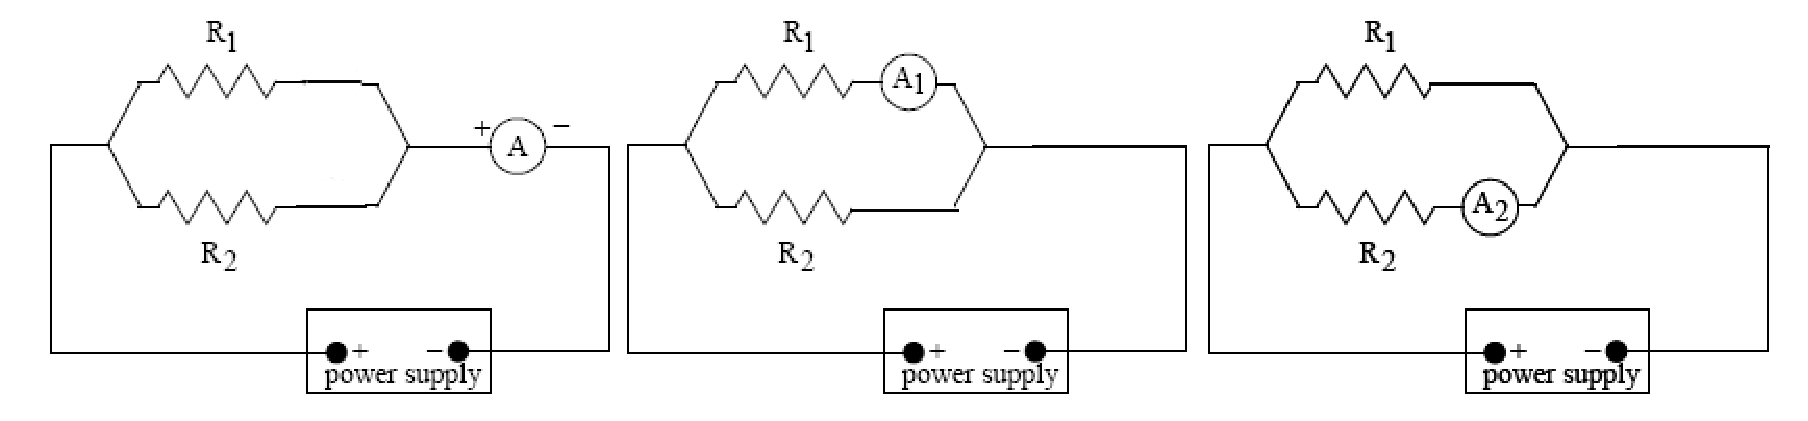
\includegraphics[width=6.0in]{ohms_law_fig_2.eps}
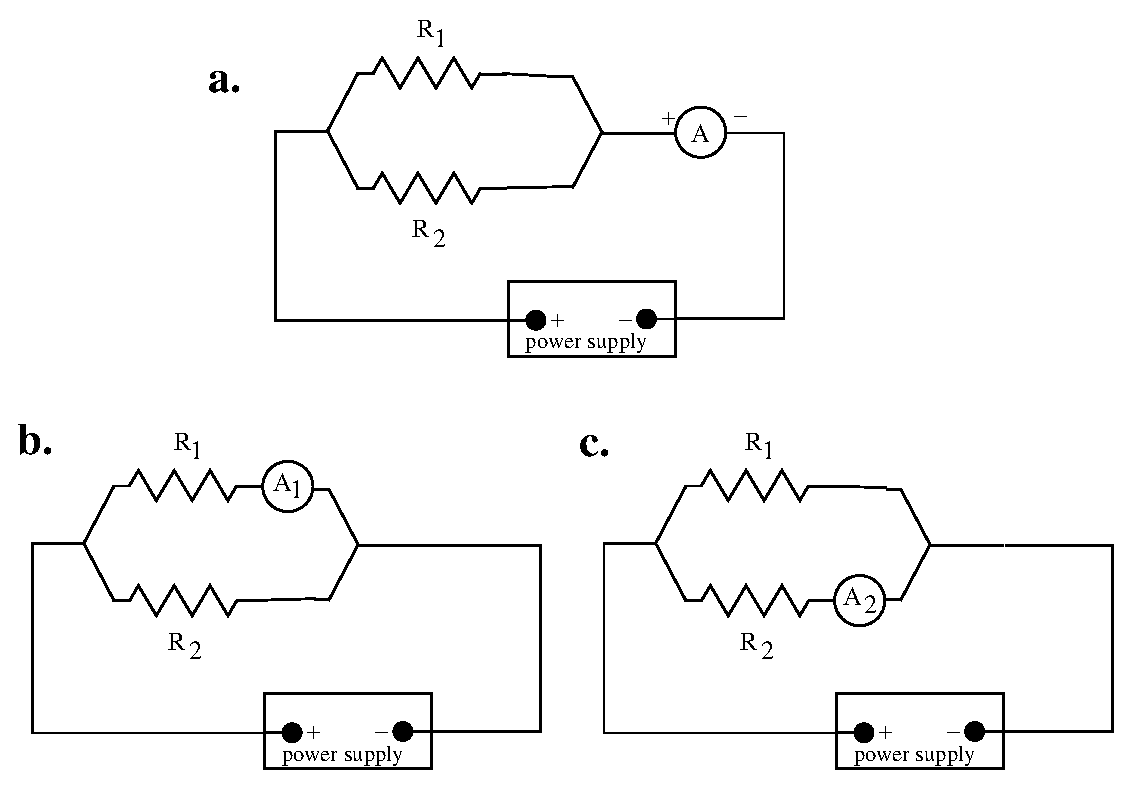
\includegraphics[width=4.6in]{ohms_law/ohms_law_fig_2b.eps}
\end{center}
\vspace{0.3cm}

\begin{itemize}
\item When you are sure the circuit is set up correctly, turn on the power 
supply and turn the coarse voltage control up to about 10 volts. Record the 
total current through the circuit and the voltage across 
the parallel resistance combination. Also measure the voltage across the 
milliammeter (which may be in millivolts). Turn off the power supply.
\vspace{20mm}

\item Connect the milliammeter to the point marked A\( _{1} \) in figure 
\textbf{b} above, without disturbing the rest of the circuit. Turn on the 
 power supply and 
record the current through R\( _{1} \) and the voltage across the parallel 
combination. Turn off the power supply.
\vspace{20mm}

\item Repeat the above measurements for R\( _{2} \), connecting the 
milliammeter at A\( _{2} \) as in figure \textbf{c} above. Turn off the 
power supply.
\vspace{20mm}

%\item Using Ohm's Law, calculate the two resistances of the parallel connection
%and also the total resistance of the circuit. Check with the ohmmeter
%and determine the percent differences.\vspace{30mm}

\item What is the relationship between the total current and the current
in each of the branches of the parallel circuit? (This is an example of 
Kirchhoff's junction rule which is based on conservation of charge.)
\vspace{30mm}

\item Using Ohm's Law and your data above, calculate the resistance of each 
resistor and the total resistance of the circuit.
\vspace{60mm}

\item What is the relationship between the total resistance of the parallel
circuit and the resistance of each of the branches? Using this relationship, 
calculate the total resistance of the circuit from the individual resistances 
you determined above. Does the result agree with what you calculated in the 
previous item? Calculate a percent difference and record it here.


%\item Determine, using Ohm's law, what the voltage was in each branch of
%the parallel circuit. Did it make any difference that you didn't reposition
%the voltmeter during this activity? On the basis of Ohm's law, does
%the result make sense?\vspace{30mm}

%\item Can the total resistance of a series combination ever be less than
%the resistance of the largest resistor? Explain.\vspace{30mm}

%\item Can the total resistance of a parallel combination ever be greater
%than the resistance of the smallest resistor? Explain.\vspace{30mm}
\end{itemize}

